\documentclass[a4paper,12pt,oneside,final]{report}
\usepackage[pdftex]{graphicx}
\usepackage{amssymb}
\usepackage{epstopdf}
\usepackage[utf8]{inputenc}
\usepackage{titlesec}
\usepackage[titletoc]{appendix}
\titleformat{\chapter}[hang]{\bf\Huge}{\thechapter}{1cm}{}

\usepackage[colorlinks=true]{hyperref}
\hypersetup{urlcolor=blue,linkcolor=black,citecolor=black,colorlinks=true}
\bibliographystyle{plain}

\pagestyle{plain}
% -------------------- this stuff for code --------------------

\usepackage{anysize}
\marginsize{30mm}{30mm}{20mm}{20mm}

\newenvironment{formal}{%
  \def\FrameCommand{%
    \hspace{1pt}%
    {\color{blue}\vrule width 2pt}%
    {\color{formalshade}\vrule width 4pt}%
    \colorbox{formalshade}%
  }%
  \MakeFramed{\advance\hsize-\width\FrameRestore}%
  \noindent\hspace{-4.55pt}% disable indenting first paragraph
  \begin{adjustwidth}{}{7pt}%
  \vspace{2pt}\vspace{2pt}%
}
{%
  \vspace{2pt}\end{adjustwidth}\endMakeFramed%
}

\newenvironment{changemargin}[2]{\begin{list}{}{%
\setlength{\topsep}{0pt}%
\setlength{\leftmargin}{0pt}%
\setlength{\rightmargin}{0pt}%
\setlength{\listparindent}{\parindent}%
\setlength{\itemindent}{\parindent}%
\setlength{\parsep}{0pt plus 1pt}%
\addtolength{\leftmargin}{#1}%
\addtolength{\rightmargin}{#2}%
}\item }{\end{list}}

\usepackage{color}
\usepackage{dsfont}
\usepackage[bitstream-charter]{mathdesign}
\usepackage[scaled]{helvet}
\usepackage{inconsolata}


\definecolor{colKeys}{rgb}{0,0,0.9} 
\definecolor{colIdentifier}{rgb}{0,0,0} 
\definecolor{colString}{rgb}{0.7,0,0} 
\definecolor{colComments}{rgb}{0,0.6,0} 
\usepackage{listings}
\lstset{
  stringstyle=\color{colString},
  keywordstyle=\color{colKeys},
  identifierstyle=\color{colIdentifier},
  commentstyle=\color{colComments},
  numbers=left,
  tabsize=4,
  frame=single,
  breaklines=true,
  basicstyle=\small\ttfamily,
  numberstyle=\tiny\ttfamily,
  framexleftmargin=0mm,
  xleftmargin=7mm,
  xrightmargin=7mm,
  frameround={tttt},
  captionpos=b
}

\usepackage{mathtools}
\usepackage{amsthm}
\newtheorem{definition}{Definition}
\newtheorem{theorem}{Theorem}
\DeclareMathOperator*{\argmin}{ArgMin\ }
\DeclareMathOperator*{\argmax}{ArgMax\ }

\usepackage{algorithm}
\usepackage{algorithmic}

\usepackage[usenames,dvipsnames]{xcolor}
\makeatletter
\DeclareRobustCommand{\em}{%
  \@nomath\em \if b\expandafter\@car\f@series\@nil
  \normalfont \else \bfseries \fi}
\makeatother

%% Headers and footers
\usepackage{fancyhdr}
\usepackage[section]{placeins}
\pagestyle{fancy}
\fancyhf{}
\addtolength{\headwidth}{30pt}
\addtolength{\headwidth}{30pt}
\renewcommand{\headrulewidth}{0.4pt} % thickness of the header line
\renewcommand{\footrulewidth}{0.4pt} % thickness of the footer line
\renewcommand{\chaptermark}[1]{\markboth{#1}{#1}} % chapter name
\renewcommand{\sectionmark}[1]{\markright{\thesection\ #1}}  % section name
\lhead[\fancyplain{}{\bf\thepage}]{\fancyplain{}{\bf\rightmark}} % display header
\rhead[\fancyplain{}{\bf\leftmark}]{\fancyplain{}{}} % display header
\fancyfoot[C]{\bf\thepage} % display footer (page number)
\fancyfoot[R]{\bf\today} % display footer (date)
\fancypagestyle{plain}{ 
	\fancyhead{} \renewcommand{\headrulewidth}{0pt}
}
\newcommand{\clearemptydoublepage}{\newpage{\pagestyle{plain}\cleardoublepage}}

\usepackage[T1]{fontenc}
\usepackage{enumerate}
\usepackage{afterpage,lastpage,fancyhdr}
\usepackage[includeheadfoot,margin=2.5cm]{geometry}
\geometry{letterpaper}                   % ... or a4paper or a5paper or ... 

\DeclareGraphicsRule{.tif}{png}{.png}{`convert #1 `dirname #1`/`basename #1 .tif`.png}

\makeatletter \def\thickhrulefill{\leavevmode \leaders \hrule height 1pt\hfill
\kern \z@} \renewcommand{\maketitle}{
    \begin{titlepage}
    \let\footnotesize\small \let\footnoterule\relax \parindent \z@ \reset@font
    \null\vfil
    \vspace{-20mm}
    \begin{center}
    {\small \scshape Imperial College London \\ Department of Computing}
    \end{center}
    \vspace{0.5cm}
	\begin{minipage}{\textwidth}
		\vspace{1cm}
		\noindent\rule[0ex]{\textwidth}{4pt} \\
		\flushright
		\center
		\@title
		\\ \vspace{4mm}
		\noindent\rule[0ex]{\textwidth}{4pt} \\
	\end{minipage}
	\vspace{1.5cm}
	\begin{minipage}{\textwidth}
		\flushright
		{\bfseries}
		\vspace{7mm}
		\center
		\@author.\\
	\end{minipage}
	\vspace{0.5cm}
	\begin{center}
		
\includegraphics[width=70mm,]{logo_imperial_college_london.png}
	\end{center}
	\vspace{\stretch{1}}
	\vspace{50mm}
		\flushleft
		{\bfseries}
		Module leader \& Lecturer: Dr Maja \textsc{Pantic}. \\
		{\small \scshape \@date }.
		\vspace{0.1cm}
		\rule{\linewidth}{.5pt}
  \end{titlepage}
  \setcounter{footnote}{1}
  \setcounter{page}{2}
}


\author{
    Sedef Ozlen (so512, s5) \\ 
    Paul Gribelyuk (pg1312, a5) \\
    Jean Kossaifi (jk712, a5) \\ 
    Romain Brault (rb812, a5)
}
\makeatother
\title{\Huge Machine Learning \\ Case Based Reasoning \\ Coursework 4}
\date{\today}


\usepackage{amsmath}
\begin{document}
\maketitle
\tableofcontents
\listoffigures

\chapter{Introduction}
The purpose of the Case-Based Reasoning was to gain familiarity with the classification algorithm based on a similarity measure and a database of examples to compare new data with.  The critical component was to implement an intelligent structure to store and access the data when performing classification.  We found that the algorithm forces a tradeoff between performance and accuracy since clustering, the solution we chose, allows us to narrow down the set of cases to search through at the cost of misclassifying a small percentage of data.  
Through this module, we learned that \emph{lazy learning} can be applied to infer information by blurring the training and the classification stage of the machine learning process.  By continuously adding new data to the database of cases, we are able to improve the classification rate as the machine is presented with previously unseen examples.

\chapter{Implementation of CBR}
\paragraph{}
The first stage of CBR is to create an initial database of cases (case base).  We do this with the following MATLAB call:
\begin{changemargin}{-5mm}{-5mm}
\begin{lstlisting}[language=Matlab, frame=single]
case_base = CBRinit(x, y)
\end{lstlisting}
\end{changemargin}
where \verb+x+ and \verb+y+ are initial cases with their correct classifications, respectively.  We split this data according to their class, creating a bucket within the case base in the following way:
\begin{changemargin}{-5mm}{-5mm}
\begin{lstlisting}[language=Matlab, frame=single]
CBR.base{i}.vector = CaseStr.empty;
CBR.base{i}.count = 0;
CBR.base{i}.meanVec = zeros(1,size(x,2));
\end{lstlisting}
\end{changemargin}
where the \verb+vector+ field contains a list of \verb+CaseStr+ objects, the \verb+count+ field is the number of cases in that cluster, and the \verb+meanVec+ field stores the average action unit (AU) example associated with that cluster.  
We represent a case (\verb+CaseStr+ in our code), as an object with the properties:
\begin{changemargin}{-5mm}{-5mm}
\begin{lstlisting}[language=Matlab, frame=single]
properties
  activeAU;
  solution;
  timesRetrieved = 0;
  cbrIndex;
end
\end{lstlisting}
\end{changemargin}
storing the indices of the active AUs, the class associated with that case, and the typicality of the case.  We instantiate a \verb+caseStr+ from an example row in the following manner:
\begin{changemargin}{-5mm}{-5mm}
\begin{lstlisting}[language=Matlab, frame=single]
z = CaseStr(example, solution);
\end{lstlisting}
\end{changemargin}
where the \verb+solution+ argument is optional for the situations when we create case instances without available solutions.

\begin{itemize}
\item {\bf\textit{Minkowski:}} $d(a,b) = \sqrt[r]{\sum_i (a_i - b_i)^r}$
\item {\bf\textit{Manhattan:}} $d(a,b) = \sum_i (a_i - b_i)$
\item {\bf\textit{commonality:}} number of same active AUs $d_C(a, b) = \|\{(a_i, b_i) \quad such\; that \quad a_i = b_i\}\|$
\item {\bf\textit{activity:}} absolute difference in number of active AUs $d_A(a,b) = |d_{NYC}(0, a) - d_{NYC}(0, b)|$
\item {\bf\textit{Clark:}} $d(a, b) = \sqrt{\sum_i \left( \frac{|a_i - b_i|}{a_i + b_i} \right)^2}$
\item {\bf\textit{Canberra:}} $d(a, b) = \sum_i \frac{|a_i - b_i|}{a_i + b_i}$
\item {\bf\textit{Earth Mover Distance:}} Answers the question: "how much work should be done to convert from one example to another?" We found this distance measure to be very appropriate for the problem, unfortunately, no quickly available solution was available and we did not have time to implement the entire minimization function.  However, we believe this bears further consideration.
\end{itemize}
Since some of these are measures of distance, we could either choose to minimize it when searching for a best case or maximize the similarity as defined by $1 - {d(a,b)}/M$, where $M$ is the maximum value the distance can possibly take.

\paragraph{}
Our \verb+retrieve+ algorithm iterates over the clusters previously instantiated in the \verb+CBRinit+ function call and finds the cluster for which, the similarity between a new example and the \verb+meanVec+  
\paragraph{}
Our implementation of the \verb+retain+ step in CBR checks if the case being added has already been encountered.  If so, we simply increment the count and update our \verb+meanVec+ variable to reflect the added weight due to that combination of AUs.  However, we do not add it as a unique case to our case base, as it would be redundant.  If the case is unique to our case base, then the \verb+CBR.base{class}.vector+ list is updated with this new case (as well as updating the other variables).  In the situation that a case already existed in the case base when retaining it, we treated it as a separate case.  This produce no problems, since our implementation of \verb+retrieve+ will uniquely identify a best case, and if two are tied (e.g. if they are the same case), then it will return a random one.  We also update the \verb+meanVec+ field for the corresponding cluster, thus giving more weight to those attributes.

We implemented the \verb+retrieve+ algorithm by considering the similarity between the AU-representation of a \verb+newCase+ and the \verb+meanVec+ field of a CBR cluster.  This allowed us to make very few similarity comparisons per example while narrowing down the results quickly.  To account for cases when two or more clusters tie for most similar, we compared the \verb+timesRetrieved+ field for each case in each of the tied clusters, and, if more than one case remained, we chose randomly.

The implementation of the \verb+reuse+ method is extremely straightforward and is available in the code.

\chapter{Cross-Validation}
\paragraph{}
To properly cross-validate the performance of our CBR it was first necessary to write a special cross-validation method to make sure that the data passed into \verb+CBRInit+ contains at least one example from each class.  To do this, we implemented a startification technique in the \verb+stratifiedKFold+ method.  

\paragraph{}
Obtaining results from the CBR is a three-fold process for us, and is implemented as follows:
\begin{changemargin}{-5mm}{-5mm}
\begin{lstlisting}[language=Matlab, frame=single]
n = size(testData, 1);
y = zeros(n, 1);
% For every example (ie every row of testData)
% Retrive the nearest neighbour, Reuse it, Retain the row    
for i = 1:n
  c = createCase(testData(i, :));
  bestCase = retrieve(cbr, c);
  y(i) = bestCase.solution;
  caseToRetain = reuse(bestCase, c);
  cbr = retain(cbr, caseToRetain);
end
\end{lstlisting}
\end{changemargin}
Clearly, we chose to use lazy learning to enhance the results of this method over time, since we "retain" examples that have already been classified.  However, this is not always optimal since misclassifications can lead to further misclassifications with little to prevent the model from gradually becoming less accurate with data.  One approach to ameliorate this would be to retain only those points which we can classify with a high degree of confience (as measure by our similarity measure).  Alternatively, we could add these new cases, but reflect the uncertainty of their class by creating a weights system and assigning them lower weights (for example in the \verb+meanVec+ field).

\paragraph{}
Next, we considered four different similarity measures and obtained the following error rates using 10-fold cross-validation:
\begin{verbatim}
modifiedManhattan = 21.62%
modifiedMinkowski (r=2) = 18.30%
Commonality = 20.98%
Canberra = 15.58%
\end{verbatim}
We alse obtained the following precision:
\begin{verbatim}
modifiedManhattan = 76.29%
modifiedMinkowski (r=2) = 79.68%
Commonality = 75.31%
Canberra = 84.91%
\end{verbatim}
recall:
\begin{verbatim}
modifiedManhattan = 76.28%
modifiedMinkowski (r=2) = 81.56%
Commonality = 76.22%
Canberra = 81.79%
\end{verbatim}
and $F_1$ measures:
\begin{verbatim}
modifiedManhattan = 75.49%
modifiedMinkowski (r=2) = 78.54%
Commonality = 75.74%
Canberra = 79.51%
\end{verbatim}
with these average confusion matrices (number of outcomes):
\[
Manhattan = \left[\begin{array}{cccccc}
   10.6000 &   0.8000 &   1.0000 &   0.3000 &   0.2000 &   0.3000\\
    2.8000 &  13.7000 &   0.7000 &   1.3000 &   0.8000 &   0.5000\\
    0.5000 &   0.2000 &   9.2000 &   0.4000 &        0 &   1.6000\\
         0 &   0.1000 &   0.3000 &  21.0000 &        0 &   0.2000\\
    2.9000 &   1.7000 &   1.2000 &   0.7000 &   5.9000 &   0.8000\\
    0.1000 &   0.2000 &   1.3000 &   0.7000 &   0.1000 &  18.3000\\
\end{array}
\right]
\]

\[
Minkowski = \left[\begin{array}{cccccc}
   10.9000 &   0.5000 &   1.0000 &   0.1000 &   0.5000 &   0.2000\\
    3.0000 &  13.4000 &   0.7000 &   1.1000 &   1.3000 &   0.3000\\
    0.3000 &   0.1000 &  10.8000 &   0.1000 &   0.1000 &   0.5000\\
    0.1000 &   0.1000 &   0.4000 &  20.7000 &        0 &   0.3000\\
    2.3000 &   1.2000 &   0.8000 &   0.4000 &   8.1000 &   0.4000\\
    0.1000 &   0.1000 &   1.3000 &   0.4000 &   0.1000 &  18.7000\\
\end{array}
\right]
\]

\[
Commonality = \left[\begin{array}{cccccc}
   10.0000 &   0.8000  &  0.8000 &   0.2000  &  1.2000  &  0.2000\\
    1.3000 &  16.7000  &  0.8000 &   0.5000  &  0.3000  &  0.2000\\
    0.4000 &   0.4000  &  8.4000 &   0.7000  &  1.0000  &  1.0000\\
    0.1000 &   0.5000  &  0.1000 &  20.6000  &  0.2000  &  0.1000\\
    2.2000 &   3.8000  &  0.3000 &   0.4000  &  6.2000  &  0.3000\\
         0 &   0.1000  &  1.3000 &   1.0000  &  0.8000  & 17.5000\\
\end{array}
\right]
\]

\[
Canberra = \left[\begin{array}{cccccc}
7.8000  &  1.7000 &   1.3000  &  0.9000  &  1.2000 &   0.3000 \\
    0.5000 &  16.9000 &   0.5000 &   1.1000   & 0.8000  &       0 \\
         0 &   0.1000 &  10.4000 &   0.2000   & 0.3000  &  0.9000 \\
         0 &   0.1000 &        0 &  21.4000   &      0  &  0.1000 \\
    0.4000 &   2.8000 &   0.5000 &   0.6000   & 8.6000  &  0.3000 \\
         0 &        0 &   0.5000 &   0.4000   &      0  & 19.8000 \\
\end{array}
\right]
\]

\chapter{Questions}
\begin{itemize}
\item[1] We solved the problem of finding multiple "best matches" by adding a field to our implementation of a case object which counts how many times this item has been retrieved to help classify an example.  Those which have been best cases in the past will tend to be in the future as well.  If more than one case remained, we chose randomly.  However, since we used clustering, the initial step of comparing with an average vector for each class ensures that there is a very low probability of having more than one best match.  Alternatively, applying another similarity measure to determine a best case would also be an interesting approach.
\item[2]  When adding an example which is aready in the CBR, we added it to our database and updated the \verb+meanVec+ and \verb+count+ fields for that cluster accordingly.  We believe this is not a problem to do since the algorithm for selecting a best case can handle situations of more than one "best case".
\item[3]  We have outlined the similarity measures above.  We used:
\begin{itemize}
\item the modified manhattan - only using top ten active activation unite in comparing the example with \verb+meanVec+; This has the advantage of working well on discrete data, and being able to provide a good variety of "best cases" for further filtering.
\item the modified Minkowski with $r = 2$ (Euclidean) - again taking the top $K$ active units in the attribute data; This is the standard metric and has the added quality that it is tractable and easy to optimize
\item Commonality - this measure also works well on discrete (rather than continous) data.  However, since we are averaging the examples in each cluster to get a representative example, this has limited use.  If we chose a representative sample (or a collection of representatives) differently, this measure would like fare best.
\item Canberra - provides a pointwise difference as a percentage of the total spread of the data;  this only works when attributes are greater than zero, so we had to increase the AU vectors by $1$ to allow this to work.
\end{itemize}
\item[4]  We initialized the CBR system by adding initial data to clusters based on the target class for that data and updating a few characteristic values per cluster.  
\item[5] CBR belongs to the class of \emph{lazy learning} algorithms.  This approach also crosses over to unsupervised learning, since having a solution is not always required (i.e. we can simply group by similarity, without knowing what that grouping means).  Unlike Neural Networks or Decision Trees, CBR does not have to rely on models with a large number of assumptions.  Furthermore, CBR algorithms can perpetually train on new data, thus making them more viable temporally.
\end{itemize}

\chapter{An Alternative CBR model - KNN}
We wanted to see if a simple KNN (K-nearest neighbors) model would produce better results than our more sophisticated clustering and retrieval algorithms above.  Our implementation contains two files, one for training:
\begin{changemargin}{-5mm}{-5mm}
\begin{lstlisting}[language=Matlab, frame=single]
function params = basicKNNtrain(X, y)
%basicKNNtrain
    params.X = X;
    params.y = y;
    params.K = 6; % number of neighbours
    params.distance = 'manhattan';
end
\end{lstlisting}
\end{changemargin}
essentially storing the input values, and the other for retrieval and classification, which is significantly more involved.  This approach was not only more accurate, generating a classification error of $12.63\%$.  For small datasets, small number of classes, and with a relatively inefficient language like MATLAB, KNN is preferable to our clustering algorithm.  However, we believe that it scales better with more data.  Furthermore, if retrieval was equally computationally intesnive (currently objects and cells are the limiting reagent), there would be a computational advantage to using these clustering techniques since we could confidently narrow down our search space.


% \section{}
% \paragraph{}


% \begin{figure}[!h]
% \begin{changemargin}{-20mm}{-20mm}
% \center
% %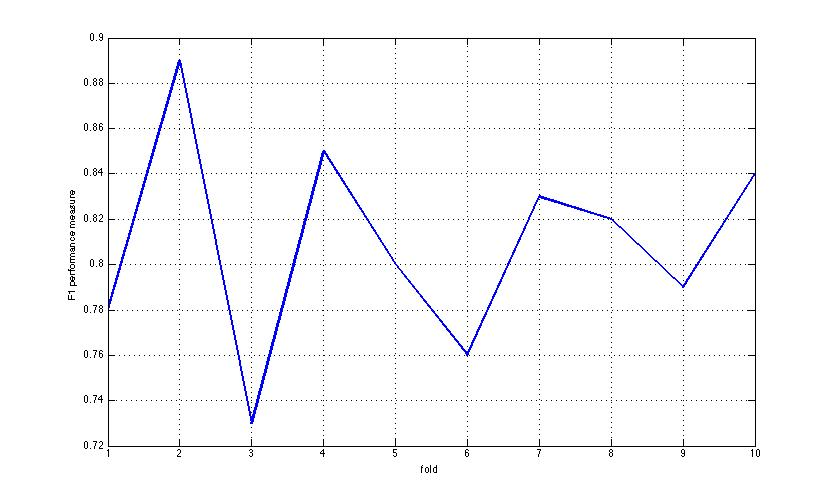
\includegraphics[scale=0.5]{single_perf.jpg}
% \caption{A figure caption}
% \end{changemargin}
% \end{figure}

% \paragraph{}
% \chapter{Conclusion}
% \paragraph{}

\bibliographystyle{alpha}
\bibliography{biblio.bib}

\begin{appendices}

\end{appendices}

\end{document}  
